%%% ---- PACKAGES ---

% I use a lot of Packages. 
\usepackage{etex}

%Math Packages	
\usepackage{amssymb}	%Common Math Symbols
\usepackage{tikz}[external]	%Vector Graphics
\usepackage{tikz-cd}	%Commutative Diagrams
\usepackage{import}
\usetikzlibrary{matrix,arrows,  decorations.markings,  patterns,  plotmarks, calc}	%Special types of vector graphics you may want
\usepackage{amsmath}	%Useful math commands
%\usepackage{mathtools}
\usepackage{verbatim}	%Allows you to create big comments
\usepackage{environ}
\usepackage{mdframed}
\usepackage{changepage}
\strictpagecheck
\usepackage{marginnote} %Does what you think it does
\usepackage{etoolbox}
\usepackage{afterpage}
\usepackage{fontspec}
\usepackage{fourier}

\usepackage[final]{microtype} % Less badboxes


%%% Indexing and Things

\usepackage{makeidx}	%Makes and Index
\usepackage[backend=bibtex, style=alphabetic, maxcitenames=5, maxbibnames=9 ]{biblatex}	%Advance version of bibliography, with commands on how I want that bibliography to appear
%\usepackage{hyperref} %Make hyperlinks. This is usually the last package you should load. 
\usepackage[refpage]{nomencl} %Nomenclatures

%%%%% Sizes and Stuff


\definecolor{mycolor}{rgb}{0.122, 0.435, 0.698}
\def \scalefactor{1}
\newfontfamily{\stationfont}{Calibri}
\newcommand{\attractionsubtitlefont}{\scriptsize\stationfont}
\newlength{\figuretextheight}
\newlength{\tuftesize}
\newlength{\figurefigureheight}
\newlength{\figurecaptionheight}
\newlength{\thisfigurewidth}
\newlength{\intermediateheight}
\newlength{\leftoverspace}
\newlength{\tuftemargin}
\newlength{\intermediate}
\newlength{\tuftefiguresize}
\newlength{\figuretextwidth}
\newlength{\hanginglength}
\setlength{\leftoverspace}{0pt}
\setlength{\fboxsep}{0pt}
\setlength{\tuftesize}{2in}
\setlength{\hanginglength}{1cm}
\def \stationlineindent {1.1in}
\def \stationmarkerindent {1.1 in}
\def \labeloffset {10pt}
\setlength{\tuftemargin}{20pt}
\def \metrolinewidth{4pt}
\dimdef{\tuftefiguresize}{\tuftesize-\tuftemargin}
\setulmarginsandblock{1in}{*}{1}

\makechapterstyle{standard}{
	\renewcommand{\chapterheadstart}{\vspace*{\beforechapskip}}
	\renewcommand{\chapnamefont}{\normalfont\Large}
	\renewcommand{\printchaptername}{}
	\renewcommand{\chapternamenum}{}
	\renewcommand{\chapnumfont}{e}
	\renewcommand{\printchapternum}{}
	\renewcommand{\afterchapternum}{}
	\renewcommand{\printchapternonum}{}
	\renewcommand{\chaptitlefont}{}
	\renewcommand{\printchaptertitle}[1]{ }}
	\renewcommand{\afterchaptertitle}{}
	\renewcommand{\clearforchapter}{}
\makeatother
\setlrmarginsandblock{.75in}{1.5in}{*}
\checkandfixthelayout

\definecolor{shadecolor}{rgb}{.95,.95,.95}
\definecolor{framepagecolor}{rgb}{.95,.95,.95}
\newcommand{\topgraph}{red}
\newcommand{\embedded}{green}
\newcommand{\simplicial}{blue}
\newcommand{\knots}{purple}
\newcommand{\homalg}{orange}

\newcounter{lineindex}
\newcounter{myenvcntr}




%%% Replacement for tikzscale

%%% Temporary Widths
\newlength{\mywidth}
\newlength{\myheight}
\newlength{\boundingboxwidth}
\newlength{\boundingboxheight}
\setlength{\figuretextwidth}{1\textwidth minus 1\tuftesize}

\makeatletter
\newcommand*{\DivideLengths}[2]{%
	\strip@pt\dimexpr\number\numexpr\number\dimexpr#1\relax*65536/\number\dimexpr#2\relax\relax sp\relax
}
\makeatother
\newcommand{\measuresize}[1]{\smash{\rlap{\phantom{\input{#1}}}}}


\newcommand{\includegraphicswithbound}[3]
{%
	\dimdef{\leftoverspace}{0pt}%
	\setlength{\boundingboxwidth}{#2}%
	\setlength{\boundingboxheight}{#3}%
	\measuresize{#1}%
	\edef \scalefactor {\DivideLengths{\boundingboxwidth}{\mywidth}}%
	\ifdimless{\scalefactor\myheight}{\boundingboxheight}%
	{% 
	\dimdef{\leftoverspace}{0.5\dimexpr\boundingboxheight-\dimexpr\scalefactor\myheight\relax\relax }%
	\dimdef{\intermediate}{0.5\dimexpr\boundingboxwidth-\dimexpr\scalefactor\mywidth\relax\relax }%
	}
	{%
		\edef\scalefactor {\DivideLengths{\boundingboxheight}{\myheight}}%
	}%
	\vbox{%
%	\hbox{\vspace{\leftoverspace}}%
	\hbox{\hspace{\intermediate}\input{#1}}%
	\hbox{\vspace{\leftoverspace}}%
	}%
}






%%% PAGE LAYOUT 

%%% SECTIONAL DIVISIONS

\maxsecnumdepth{subsection} % Subsections (and higher) are numbered
\setsecnumdepth{subsection}
\makeatletter %This command changes the escape keys so you can use macros inside of the next section

\chapterstyle{standard}

\setsecheadstyle{\normalfont\large\bfseries}
\setsubsecheadstyle{\normalfont\normalsize\bfseries}
\setparaheadstyle{\normalfont\normalsize\bfseries}
\setlength{\parindent}{0pt}
\nonzeroparskip



%%%  New environments and document related commands


% computes width and height of tikzpicture
\makeatletter
\newcommand{\pgfsize}{ % #1 = width, #2 = height
	\pgfextractx{\@tempdima}{\pgfpointdiff{\pgfpointanchor{current bounding box}{south west}}
		{\pgfpointanchor{current bounding box}{north east}}}
	\global\mywidth=\@tempdima
	\pgfextracty{\@tempdima}{\pgfpointdiff{\pgfpointanchor{current bounding box}{south west}}
		{\pgfpointanchor{current bounding box}{north east}}}
	\global\myheight=\@tempdima
}
\makeatother



%%% FLOATS AND CAPTIONS
\makeatletter                  % You do not need to write [htpb] all the time
\renewcommand\fps@figure{htbp} %
\renewcommand\fps@table{htbp}  %
\makeatother                   %

\captiondelim{\space } % A space between caption name and text
\captionnamefont{\small\bfseries} % Font of the caption name
\captiontitlefont{\small\normalfont} % Font of the caption text



%%% HEADER AND FOOTER 

\makepagestyle{standard} % Make standard pagestyle

\makepsmarks{standard}
{
	\createmark{chapter}{both}{shownumber}{ }{ \quad }
	\createmark{section}{right}{shownumber}{}{ \quad }
	\createplainmark{toc}{both}{\contentsname}
	\createplainmark{lof}{both}{\listfigurename}
	\createplainmark{lot}{both}{\listtablename}
	\createplainmark{bib}{both}{\bibname}
	\createplainmark{index}{both}{\indexname}
	\createplainmark{glossary}{both}{\glossaryname}
}

\makeatother                               %

\makepagestyle{chap} % Make new chapter pagestyle

\makeatletter
\makeevenhead{chap}{}{}{}   %
\makeoddhead{chap}{}{}{}    %
\makeatother

\nouppercaseheads
\pagestyle{standard}               % Choosing pagestyle and chapter pagestyle
\aliaspagestyle{chapter}{chap} %

%%% Bullets
\def\labelitemi{--}

%%% Document Indexing
\maxtocdepth{subsection} % Only parts, chapters and sections subsections in the table of contents
\settocdepth{subsection}
\AtEndDocument{\addtocontents{toc}{\par}} % Add a \par to the end of the TOC



\newcommand{\newshadedfigureenvironment}[2]%
{%
	\expandafter\NewEnviron{#1figureenv}[2][]%
	{%	
		\gdef\thismarkcode{\markcoderound}%
		\gdef\indexingtype{attraction}%
		\gdef\thisattractionwriteout{\arabic{externalattractionnumber}}%
		\gdef\thisattractionsubtitle{##1}%
		\gdef\thisattractiontype{#1}%
		\def\thisattractionexternaltype{\stationfont #2}%
		\def\thisattractionname{\itshape \attractionsubtitlefont\thisattractionsubtitle}\def\thisattractioninternallabel{}%
		\def\scalefactor{1}%
		\def\thisfigure{##2}%
		\def\thisfiguretext%
		{%
			\noindent\begin{minipage}[b]{\figuretextwidth}%
				\BODY%
			\end{minipage}%
		}%
		\if\frametoken1{%
			\xglobal\definecolor{shadecolor}{rgb}{.85,.85,.85}%
			\ifx\thisattractionsubtitle\empty{\gdef\thisattractioninternallabel{{\stationfont#2}.}}%
			\else{\gdef\thisattractioninternallabel{{\stationfont#2} (\textit{\footnotesize\stationfont\thisattractionsubtitle}). }}%
			\fi{}%			
			\gdef\thisattractionname{}%
			\gdef\thisattractionexternaltype{}%	
			\stepcounter{framedattractionnumber}%
			\gdef\thisattractionnumber{\alph{framedattractionnumber}}%
			\gdef\thisattractionwriteout{\arabic{externalattractionnumber}\alph{framedattractionnumber}}%
			\gdef\thismarkcode{\markcodesubattraction}%
		}
		\else%
		{\stepcounter{externalattractionnumber}%
		\stepcounter{attractionindex}%
		\immediate\write\myoutput{%
		\noexpand\expandafter\csname def \endcsname \noexpand\csname attractiondata@\arabic{attractionindex}\noexpand\endcsname{%
			{\thisattractionwriteout}%
			{\thisattractiontype}
			{\thisattractionsubtitle}%
			{\thelineindex}%
			{\thepage}%
			{\thismarkcode}%
			}}}%
		\fi%
		\settoheight{\figuretextheight}{\vbox{\thisfiguretext}}%
		\dimdef{\tuftefigureheight}{\dimexpr\figuretextheight-\tuftemargin\relax}%
		\def\thisincludegraphic {\includegraphicswithbound{\thisfigure}{\tuftefiguresize}{\tuftefigureheight}}%
		\leavevmode%
		\begin{shaded}%
		\checkoddpage%
		\ifoddpage%
			{%
			\hbox{%
			\begin{minipage}[b]{\figuretextwidth}{\if\frametoken0{\stationmarginmark}\fi{}\thisattractioninternallabel\BODY}\end{minipage}%
			\vtop{\hbox to \tuftesize{\hfil\thisincludegraphic\hfil}}}%
			}
		\else%
			{%	
			\hbox{{\vtop{%
				\vbox{\hbox to \tuftesize{\hfil\thisincludegraphic\hfil}}}}%
				\begin{minipage}[b]{\figuretextwidth}{\if\frametoken0{\stationmarginmark}\fi{}\thisattractioninternallabel \BODY}\end{minipage}%	%
			}%
			}%
		\fi%
				\end{shaded}%
				\xglobal\definecolor{shadecolor}{rgb}{.95,.95,.95}%
	}%
}%
		\def\includefigure#1{\par\begin{center}\includegraphicswithbound{#1}{\textwidth}{3.5cm}\end{center}\par}
\newcommand{\newfigureenvironment}[2]%
{%	
	\expandafter \def \csname catcode#1\endcsname{0}%
	\expandafter\NewEnviron{#1figureenv}[2][]%
	{\par%
		\def \scalefactor{1}%
		\def \thistitle{\textit{\stationfont ##1}}%
		\def \thisfigure{##2}%
		\def \thisfiguretext%
		{%
			\noindent\begin{minipage}[b]{\figuretextwidth}%
				\BODY%
			\end{minipage}%
		}%
		\def \thisfiguretextl%
		{%
			\noindent\parbox[b]{\figuretextwidth}{\BODY}%
		}%
		\settoheight{\figuretextheight}{\vbox{\thisfiguretext}}%
		\dimdef{\tuftefigureheight}{\dimexpr\figuretextheight-\tuftemargin\relax}%
		\def \thisincludegraphic {\includegraphicswithbound{\thisfigure}{\tuftefiguresize}{\tuftefigureheight}}%
		\checkoddpage%
		\ifoddpage%
			{%
			\noindent%
			\hbox{{\begin{minipage}[b]{\figuretextwidth}{\thistitle \BODY}\end{minipage}}%
			\vbox{\begin{minipage}[b]{\tuftesize}\centering\thisincludegraphic\end{minipage}}%
			}%
			}%
		\else%
			{%
			\hbox{	\vbox{\hbox to \tuftesize{\hfil\thisincludegraphic\hfil}}%
				\begin{minipage}[b]{\figuretextwidth}{\thistitle\BODY}\end{minipage}%	
			}%
			}%
		\fi{}%
		%\\Figure Height: \tuftefigureheight\\
		%Caption Height:\the\figurecaptionheight\\
		%Text Height \the\figuretextheight\\
	}%
}%


\newcounter{attractionindex}
\newcounter{externalattractionnumber}[lineindex]
\newcounter{framedattractionnumber}[externalattractionnumber]
\newcounter{problemsetnumber}
\makeatletter
\newcommand*{\shifttext}[2]{%
  \settowidth{\@tempdima}{#2}%
  \makebox[\@tempdima]{\hspace*{#1}#2}%
}
\makeatother
\renewcommand{\newtheorem}[3][externalattractionnumber]
{	%
	\gdef\indexingtype{attraction}%
	\message{Defined newtheorem Named #2 with counter #1}%
	\expandafter \def \csname catcode#1\endcsname{0}%
	\newenvironment{#2}[1][]
	{%
	\gdef\thisattractionsubtitle{##1}
	\gdef\thismarkcode{\markcoderound}
	\gdef\thisattractiontype{#2}
	\def\thisattractionexternaltype{\stationfont #3}%
	\def\thisattractionname{\itshape \attractionsubtitlefont \thisattractionsubtitle}%
	\def\thisattractioninternallabel{}%
	\def\thisattractionnumber{\textbf {\stationfont \arabic{#1}}}%
	\def\thisattractionwriteout{\arabic{#1}}%
	\leavevmode%
	\if\frametoken1{
		\xglobal\definecolor{shadecolor}{rgb}{.85,.85,.85}%
			\ifx\thisattractionsubtitle\empty{\gdef\thisattractioninternallabel{{\stationfont#3.}}}%
			\else{\gdef\thisattractioninternallabel{{\stationfont#3} (\textit{\footnotesize\stationfont\thisattractionsubtitle}). }}%
			\fi{}%	
		\gdef\thisattractionname{}%
		\gdef\thisattractionexternaltype{}%	
		\global\stepcounter{framedattractionnumber}%
		\gdef\thisattractionnumber{\textbf{\stationfont\alph{framedattractionnumber}}}%
		\gdef\thisattractionwriteout{\noexpand\miniscule\arabic{#1}\alph{framedattractionnumber}}%
		\gdef\thismarkcode{\markcodesubattraction}
	}\fi%
	\if\frametoken2{
		\gdef\thismarkcode{\markcodeproblem}%
		}
	\fi%
	\def\FrameCommand{\fboxsep=\FrameSep \colorbox{shadecolor}}%
  \MakeFramed 
		\checkoddpage%
		\if\frametoken1{}
		\else{%
			\refstepcounter{attractionindex}%
			\stepcounter{#1}%
			\stationmarginmark
		\immediate\write\myoutput{%
				\noexpand\expandafter\csname def \endcsname \noexpand\csname attractiondata@\arabic{attractionindex}\noexpand\endcsname{%
					{\thisattractionwriteout}%
					{\thisattractiontype}%
					{\thisattractionsubtitle}%
					{\thelineindex}%
					{\thepage}
					{\thismarkcode}%
					}}}\fi{}%
					\thisattractioninternallabel%
					\noindent%
}%
{\endMakeFramed%
\xglobal\definecolor{shadecolor}{rgb}{.95,.95,.95}}
}

\newfigureenvironment{paragraph}{}

\newcounter{stationindex}
\setcounter{lineindex}{0}
\setcounter{stationindex}{0}

\newenvironment{elevator}[1][\unskip]
{%
	\newpage
	\gdef\indexingtype{station}%
	\refstepcounter{section}%
	\stepcounter{stationindex} %
	\xdef\thisattractionwriteout{\arabic{section}}%
	\xdef\thisattractionsubtitle{#1}%
	\begin{shaded}%
		\noindent%
		\immediate\write\myoutput{
			\noexpand\expandafter\csname def \endcsname \noexpand\csname stationdata@\arabic{stationindex}\noexpand\endcsname{%
				{\thisattractionwriteout}%
				{station}%
				{\thisattractionsubtitle}%
				{\thelineindex}%
				{\thepage}
				{s}%
				}}%
		\textbf{\Large\stationfont#1}\\
		\noindent }
		{\end{shaded}%
		\strut\checkoddpage
		\ifoddpage
		{\begin{tikzpicture}[remember picture, overlay]
			\if\arabic{section}1
			{\fill[white] (current page.north east) rectangle ($(current page.north east) + (-\stationlineindent-4pt,-3.25cm)$) ;}\fi
			\stationmarker{\catcodestation}{+}{($(current page.north east) + (-\stationlineindent,-3.25cm)$)}{\thisattractionwriteout}
\end{tikzpicture}}
\else
		{\begin{tikzpicture}[remember picture, overlay]
			\stationmarker{\catcodestation}{+}{($(current page.north west) + (\stationlineindent,-3.25cm)$)}{\thisattractionwriteout}
\end{tikzpicture}}
		\fi
}

%%%%%%%%% END STATION %%%%%%%%%%%%%%


\newcommand{\laststation}[1]
{%
	\pagestyle{chap}
	\gdef\frametoken{2}
	\newpage
	\leavevmode
		\strut\checkoddpage
		\ifoddpage
		{\begin{tikzpicture}[remember picture, overlay]
			\tikzset{station/.style={draw,color=white, line width =2pt ,fill=\thislinecolor, circle, inner 	sep=8pt}}
			\tikzset{metroline/.style={color=white, line width=1pt, double=\thislinecolor, double distance=\metrolinewidth}}
			\draw[metroline]  ($(current page.north east) + (-\stationlineindent,0)$) -- ($(current page.north east) + (-\stationlineindent,-3.25cm)$);
			\node[station] at  ($(current page.north east) + (-\stationlineindent,-3.25cm)$) {} ;
			\node[left] at ($(current page.north east) +(-\stationlineindent-.5cm,-3.25cm)$) {\huge \textbf{\stationfont #1}};
			\node[white] at  ($(current page.north east) + (-\stationlineindent,-3.25cm)$){\textbf{\large \stationfont P}} ;
\end{tikzpicture}}
\else
		{\begin{tikzpicture}[remember picture, overlay]
			\tikzset{station/.style={draw,color=white, line width =2pt ,fill=\thislinecolor, circle, inner 	sep=8pt}}
			\tikzset{metroline/.style={color=white, line width=1pt, double=\thislinecolor, double distance=\metrolinewidth}} 
			\node[right] at ($(current page.north west) + (\stationlineindent+.5cm,-3.25cm)$) {\huge \textbf{\stationfont #1}};
			\draw[metroline]  ($(current page.north west) + (+\stationlineindent,0)$) -- ($(current page.north west) + (\stationlineindent,-3.25cm)$);
			\node[station] at  ($(current page.north west) + (\stationlineindent,-3.25cm)$) {} ;			
			\node[white] at  ($(current page.north west) + (\stationlineindent,-3.25cm)$) {\textbf{\large \stationfont P} };
\end{tikzpicture}}
		\fi\vspace{2cm}\\
}
%%%%%%%%%%%%%%%%%%%%%%%%%%%%%%%%%%%



\NewEnviron{framedpage}[3]{
	\gdef\thisattractionsubtitle{#2}
	\stepcounter{attractionindex}%
	\stepcounter{stationindex}
	\stepcounter{externalattractionnumber}%
	\gdef\thisframedattractionnumber{\arabic{externalattractionnumber}}
	\immediate\write\myoutput{%
		\noexpand\expandafter\csname def \endcsname \noexpand\csname stationdata@\arabic{stationindex}\noexpand\endcsname{%
			{\thisframedattractionnumber}%
			{\thisattractiontype}
			{\thisattractionsubtitle{}}%
			{\thelineindex}%
			{\thepage}%
			{\csname catcodeframed\endcsname}%
			}}%
	\immediate\write\myoutput{
		\noexpand\expandafter\csname def \endcsname \noexpand\csname attractiondata@\arabic{attractionindex}\noexpand\endcsname{%
			{\thisframedattractionnumber}%
			{\thisattractiontype}
			{\thisattractionsubtitle}%
			{\thelineindex}%
			{\thepage}%
			{\csname markcodeframed\endcsname}%
			}}%
	\expandafter\global\expandafter\let\csname BODY@\themyenvcntr\endcsname\BODY
	\begingroup\edef\x{\endgroup\noexpand\afterpage{\noexpand\setcounter{myenvcntr}{\themyenvcntr}}}\x
	\afterpage{%
	\gdef\frametoken{1}%
	\gdef\indexingtype{attraction}%
	\begin{tikzpicture}[remember picture, overlay]
		\tikzset{metroline/.style={color=white, line width=1pt, double=\thislinecolor, double distance=\metrolinewidth}}
		\checkoddpage
		\ifoddpage
		{	\gdef\marginshift{1cm}%
			\begin{scope}[shift = {(current page.north east)}]
			\begin{scope}[xshift={-\stationlineindent}]
			\draw[metroline]  (0,0) .. controls (0,-0.5in) and (0,-0.5in) .. (-0.5in,-0.5in) .. controls (-1in,-0.5in) and 
			(-1.5in,-0.5in) .. 
			(-2in,-0.5in) .. controls 
			(-2.5in,-0.5in) and 
			(-2.5in,-0.5in) .. 
			(-2.5in,-1in);
			\end{scope}
		\end{scope}
		\begin{scope}[shift = {(current page.south east)}]
			\begin{scope}[shift={(-\stationlineindent, 0)}, yscale=-1]
			\draw[metroline]  (0,0) .. controls (0,-0.5in) and (0,-0.5in) .. (-0.5in,-0.5in) .. controls (-1in,-0.5in) and 
			(-1.5in,-0.5in) .. 
			(-2in,-0.5in) .. controls 
			(-2.5in,-0.5in) and 
			(-2.5in,-0.5in) .. 
			(-2.5in,-1in);
			\end{scope}
		\end{scope}
		}
		\else
		{%
			\gdef\marginshift{-1cm}%
			\begin{scope}[shift = {(current page.north west)}]
			\begin{scope}[xshift={\stationlineindent}, xscale = -1]
			\draw[metroline]  (0,0) .. controls (0,-0.5in) and (0,-0.5in) .. (-0.5in,-0.5in) .. controls (-1in,-0.5in) and 
			(-1.5in,-0.5in) .. 
			(-2in,-0.5in) .. controls 
			(-2.5in,-0.5in) and 
			(-2.5in,-0.5in) .. 
			(-2.5in,-1in);
			\end{scope}
		\end{scope}
		\begin{scope}[shift = {(current page.south west)}]
			\begin{scope}[shift={(\stationlineindent, 0in)}, rotate=180]
			\draw[metroline]  (0,0) .. controls (0,-0.5in) and (0,-0.5in) .. (-0.5in,-0.5in) .. controls (-1in,-0.5in) and 
			(-1.5in,-0.5in) .. 
			(-2in,-0.5in) .. controls 
			(-2.5in,-0.5in) and 
			(-2.5in,-0.5in) .. 
			(-2.5in,-1in);
			\end{scope}
		\end{scope}
		}
		\fi
			\fill[framepagecolor]  ($(current page.north west) + (.8in,-1in)$) rectangle ($(current page.south east) + (-.8in,1in)$);
			\fill[\thislinecolor!20]  ($(current page.north west) + (.8in,-1in)$) rectangle ($(current page.north east) + (-.8in,-2in)$);
			\node[right] at ($(current page.north west) + (3.5cm,-1.3in)$) {\huge \textbf{\stationfont #2}};
			\node[right] at ($(current page.north west) + (3cm,-1.7in)$) {\parbox{\outsidetextwidth}{\noindent\small{\stationfont #3}}};
			\stationmarker{\markcodeframed}{+}{($(current page.north west) + (3cm,-1.3in)$)}{\thisframedattractionnumber}
		\end{tikzpicture}%
		\thispagestyle{empty}\vspace{1in}\\
		\strut\hspace{\marginshift}\rlap{\begin{minipage}{\textwidth}
		{\begin{small}\csname BODY@\themyenvcntr\endcsname\end{small}}
		\end{minipage}}
		\gdef\frametoken{0}
		\clearpage}%
}






\newenvironment{doubledpage}[3]{
	\gdef\indexingtype{attraction}%
	\gdef\frametoken{1}%
	\cleartoverso%
	\stepcounter{stationindex}%
	\enlargethispage{-1cm}%
	\stepcounter{attractionindex}%
	\stepcounter{externalattractionnumber}%
	\gdef\thisframedattractionnumber{\arabic{externalattractionnumber}}
	\immediate\write\myoutput{
		\noexpand\expandafter\csname def \endcsname \noexpand\csname stationdata@\arabic{stationindex}\noexpand\endcsname{%
			{\thisframedattractionnumber}%
			{#1}%
			{#2}%
			{\thelineindex}%
			{\thepage}%
			{\csname catcodeframed\endcsname}%
			}}%
	\immediate\write\myoutput{
		\noexpand\expandafter\csname def \endcsname \noexpand\csname attractiondata@\arabic{attractionindex}\noexpand\endcsname{%
			{\thisframedattractionnumber}%
			{#1}%
			{#2}%
			{\thelineindex}%
			{\thepage}%
			{\csname catcodeframed\endcsname}%
			}}%
	\thispagestyle{empty}%
	\begin{tikzpicture}[remember picture, overlay]
		\tikzset{metroline/.style={color=white, line width=1pt, double=\thislinecolor, double distance=\metrolinewidth}} 
		\begin{scope}[shift = {(current page.north west)}]
			\begin{scope}[xshift={\stationlineindent}, xscale = -1]
			\draw[metroline]  (0,0) .. controls (0,-0.5in) and (0,-0.5in) .. (-0.5in,-0.5in) .. controls (-1in,-0.5in) and 
			(-1.5in,-0.5in) .. 
			(-2in,-0.5in) .. controls 
			(-2.5in,-0.5in) and 
			(-2.5in,-0.5in) .. 
			(-2.5in,-1in);
			\end{scope}
		\end{scope}
		\fill[framepagecolor]  ($(current page.north west) + (.8in,-1in)$) rectangle ($(current page.south east) + (.8in,1in)$);
		\fill[\thislinecolor!20]  ($(current page.north west) + (.8in,-1in)$) rectangle ($(current page.north east) + (0,-2in)$);
		\stationmarker{\markcodeframed}{+}{($(current page.north west) + (\stationlineindent,-1.3in)$)}{\thisframedattractionnumber}
		\node[right] at ($(current page.north west) + (4.5cm,-1.3in)$) {\huge \textbf{\stationfont #2}};
		\node[right] at ($(current page.north west) + (4.5cm,-1.7in)$) {\parbox{\outsidetextwidth}{\small{\stationfont #3}}};
	\end{tikzpicture}
	\begin{small}
		\afterpage{\begin{tikzpicture}[remember picture, overlay]
			\tikzset{metroline/.style={color=white, line width=1pt, double=\thislinecolor, double distance=\metrolinewidth}} 
			\fill[framepagecolor]  ($(current page.north west) + (-.8in,-1in)$) rectangle ($(current page.south east) + (-.8in,1in)$);
			\begin{scope}[shift = {(current page.south east)}]
				\begin{scope}[shift={(-\stationlineindent, 0)}, yscale=-1]
				\draw[metroline]  (0,0) .. controls (0,-0.5in) and (0,-0.5in) .. (-0.5in,-0.5in) .. controls (-1in,-0.5in) and 
				(-1.5in,-0.5in) .. 
				(-2in,-0.5in) .. controls 
				(-2.5in,-0.5in) and 
				(-2.5in,-0.5in) .. 
				(-2.5in,-1in);
				\end{scope}
			\end{scope}
		\end{tikzpicture}}\vspace{2cm}\par}%
		{\end{small}
	\thispagestyle{empty}%
	\gdef\frametoken{0}%
	\newpage
}



%%% Stations

\newenvironment{projectdescription}[1]{\buslineconnection{#1}}{}
%%% Stations 
\def\stationconnection#1{%
\leavevmode%
\ifcsname attractionlabel#1\endcsname{%
\expandafter\expandafter\expandafter\labelreader\csname attractionlabel#1\endcsname%
\expandafter\expandafter\expandafter\attractionreader\csname \labeltype data@\labelindex\endcsname%
\xdef\tempcolor{\csname linecolor@\thisattractionchapter\endcsname}%
\xdef\thisconnectionlabel{\stationfont \thisattractionname}%
}
\else
{\ClassWarning{ConnectionRef}{There were some undefined sreferences!}
\xdef\thisconnectionlabel{??}
\xdef\tempcolor{black}}
\fi{}%
\xdef\connectionpagestart{\thepage}%
\def\stationmarkeroffset{3pt}%
\checkoddpage%
\ifoddpage{%
	\begin{tikzpicture}[remember picture, overlay]
		\tikzset{metroline/.style={color=white, line width=1pt, double=\tempcolor, double distance=\metrolinewidth}} 
%		\fill[white] ($(current page.north east|-,0)-(\stationlineindent,0)+(3pt,0)$) rectangle (current page.north east);
		\draw[metroline, shift={($(current page.north east|-,0)-(\stationlineindent,0)+(6pt,0)$)}]   (0,0) .. controls (0,0.2) and (0,0.2) .. (0.2,0.4) .. controls (0.4,0.6) and (0.4,0.6) .. (0.6,0.8) .. controls (0.8,1) and (0.8,1) .. (1,1)(1,1) -- (4,1);
		{\draw[metroline] ($(current page.north east|-,0)-(\stationlineindent,0)+(6pt,0)$)--($(current page.south east)-(\stationlineindent,0)+(6pt,0)$);}
		%\node[above right] at ($(current page.north east|-,0)+(-\stationmarkerindent-6pt, 1)$) {\parbox[b]{2.5cm}{\raggedright\thisconnectionlabel}};
\end{tikzpicture}%
}%
\else{
	\begin{tikzpicture}[remember picture, overlay]
		\tikzset{metroline/.style={color=white, line width=1pt, double=\tempcolor, double distance=\metrolinewidth}} 
		\fill[white] ($(current page.north west|-,0)+(\stationlineindent,0)-(3pt,0)$) rectangle (current page.north west);
		
		\draw[metroline, shift={ ($(current page.north west|-,0) + (\stationlineindent,0)-(6pt, 0)$)}]  (0,0) .. controls (0,0.2) and (0,0.2) .. (-0.2,0.4) .. controls (-0.4,0.6) and (-0.4,0.6) .. (-0.6,0.8) .. controls (-0.8,1) and (-0.8,1) .. (-1,1)(-1,1) -- (-4,1);

		 
		\draw[metroline]  ($(current page.north west|-,0) + (\stationlineindent,0)-(6pt, 0)$) -- ($(current page.south west) + (\stationlineindent,0)-(6pt, 0)$);
		%\node[above right] at ($(current page.north west|-,0)+(\stationmarkerindent+6pt, 1)$) {\parbox[b]{2.5cm}{\raggedleft\thisconnectionlabel}};
\end{tikzpicture}}%
\fi{}%
\afterpage{\xdef\secondlinecolor{\tempcolor}}%
}


\def\endstationconnection{%
\def\stationmarkeroffset{0pt}%
	\checkoddpage%
	\ifoddpage{%
		\begin{tikzpicture}[remember picture, overlay]
			\tikzset{metroline/.style={color=white, line width=1pt, double=\tempcolor, double distance=\metrolinewidth}}
			\fill[white]  ($(current page.north east|-,0) - (\stationlineindent,0)+(3pt, 0)$) rectangle ($(current page.south east) - (\stationlineindent,0)+(10pt, 0)$); 
			\draw[metroline, shift={($(current page.north east|-,0)-(\stationlineindent,0)+(6pt,0)$)}]   (0,0) .. controls (0,-0.2) and (0,-0.2) .. (0.2,-0.4) .. controls (0.4,-0.6) and (0.4,-0.6) .. (0.6,-0.8) .. controls (0.8,-1) and (0.8,-1) .. (1,-1)(1,-1) -- (4,-1);
			\ifnum\connectionpagestart=\thepage
			{}
			%\else
			%{\draw[metroline] ($(current page.north east|-,0)-(\stationlineindent,0)+(6pt,0)$)--($(current page.north east)-(\stationlineindent,0)+(6pt,0)$);}
			\fi{}%
	\end{tikzpicture}%
	}%
	\else{%
		\begin{tikzpicture}[remember picture, overlay]
			   \tikzset{metroline/.style={color=white, line width=1pt, double=\tempcolor, double distance=\metrolinewidth}} 	
			   \fill[white]  ($(current page.north west|-,0) + (\stationlineindent,0)-(3pt, 0)$) rectangle ($(current page.south west) + (\stationlineindent,0)-(10pt, 0)$);	   	
			\draw[metroline, shift={ ($(current page.north west|-,0) + (\stationlineindent,0)-(6pt, 0)$)}]  (0,0) .. controls (0,-0.2) and (0,-0.2) .. (-0.2,-0.4) .. controls (-0.4,-0.6) and (-0.4,-0.6) .. (-0.6,-0.8) .. controls (-0.8,-1) and (-0.8,-1) .. (-1,-1)(-1,-1) -- (-4,-1);
			\ifnum\connectionpagestart=\thepage
{}
\else{
\draw[metroline] ($(current page.north west|-,0)+(\stationlineindent,0)-(6pt,0)$)--($(current page.north west)+(\stationlineindent,0)-(6pt,0)$);}
\fi{}%
	\end{tikzpicture}}%
	\fi{}%
\afterpage{	\xdef\tempcolor{white}%
	\xdef\secondlinecolor{white}}%
}


%%%%%%%%%%% Adding Station LInes to whole document


\usetikzlibrary[calc]
\makeevenhead{plain}{}{
    \begin{tikzpicture}[remember picture, overlay]
		   \tikzset{metroline/.style={color=white, line width=1pt, double=\thislinecolor, double distance=\metrolinewidth}} \draw[metroline]  ($(current page.north west) + (\stationlineindent,0)$) -- ($(current page.south west) + (\stationlineindent,0)$);
		   \tikzset{metroline/.style={color=white, line width=1pt, double=\secondlinecolor, double distance=\metrolinewidth}} \draw[metroline]  ($(current page.north west) + (\stationlineindent,0)-(6pt, 0)$) -- ($(current page.south west) + (\stationlineindent,0)-(6pt, 0)$);
\end{tikzpicture}}{}
\makeoddhead{plain}{}{
    \begin{tikzpicture}[remember picture, overlay]
		\tikzset{metroline/.style={color=white, line width=1pt, double=\thislinecolor, double distance=\metrolinewidth}} \draw[metroline]  ($(current page.north east) - (\stationlineindent,0)$) -- ($(current page.south east) - (\stationlineindent,0)$);
		\tikzset{metroline/.style={color=white, line width=1pt, double=\secondlinecolor, double distance=\metrolinewidth}} \draw[metroline]  ($(current page.north east) - (\stationlineindent,0)+(6pt, 0)$) -- ($(current page.south east) - (\stationlineindent,0)+(6pt, 0)$);
\end{tikzpicture}}{}
\makeevenfoot{plain}{}{\stationfont\thepage}{}
\makeoddfoot{plain}{}{\stationfont\thepage}{}
\pagestyle{plain}



%\makeevenhead{standard}{\bfseries\thepage\normalfont\qquad\small\leftmark}{}{}
%\makeoddhead{standard}{}{}{\small\rightmark\qquad\bfseries\thepage}



%% NEW TOC COMMANDS

\def\stationreader#1#2#3#4#5#6{
	\gdef \thisstationnumber{#1}
	\edef \thisstationtype{#2}
    \edef \thisstationname{#3}
    \edef \thisstationchapter{#4}
    \edef \thisstationpage{#5}
    \edef \thisstationmarkcode{#6}
    \edef \thisstationcatcode{\csname catcode\thisstationtype\endcsname}
	}
\def\stationoftype#1{
	\if\thisstationchapter\thelineindex{
    \if\thisstationcatcode#1
    {   
        \node[right] at   ( .4,-\stationspacingfactor*\the\indexintype) {\stationfont  \normalsize\thisstationname};
        \node[left] at   ( -.4,-\stationspacingfactor*\the\indexintype) {\stationfont  \normalsize\thisstationpage};
		\expandafter\gdef\csname stationtype\the\indexintype \endcsname{station}
		\global\advance \indexintype 1\relax
    }
    \else
    {	
		\node[right] at   ( .4,-\stationspacingfactor*\the\indexintype) {\textit{\stationfont \small \thisstationname}};
        \node[left] at   ( -.4,-\stationspacingfactor*\the\indexintype) {\stationfont  \normalsize\thisstationpage};
		\expandafter\gdef\csname stationtype\the\indexintype \endcsname{pagestation}
	\global\advance \indexintype 1\relax
	}
    \fi{}}\fi{}
}
\tikzset{apply style/.code={\tikzset{#1}}}


\def\indexstations#1
{
\begin{scope}[]
\newcount\dataindex
\dataindex=1
\loop
\expandafter\expandafter\expandafter\stationreader\csname stationdata@\the\dataindex\endcsname%
\stationoftype{#1}
\advance \dataindex 1\relax
\expandafter\ifx\csname stationdata@\the\dataindex\endcsname \relax
{}
\else\repeat
\draw[metroline] (0,0) -- ( 0,-\stationspacingfactor*\indexintype+\stationspacingfactor);
\advance \indexintype -1 \relax
\foreach \x in {0, ..., \indexintype}
\edef\thisindex{\x}
\edef\styleattributes{\csname stationtype\thisindex \endcsname}
\node[apply style/.expand once=\styleattributes] at (0, -\stationspacingfactor*\x) {};
\end{scope}
}



\newcommand{\chaptercontents}[3]{%

\input{#2}
	\thispagestyle{empty}%
	\gdef\frametoken{0}%
	\stepcounter{lineindex}%
	\setcounter{section}{0}%
	\xdef\thislinecolor{\csname linecolor@\thelineindex\endcsname}
	\gdef\indexingtype{line}%
	\gdef\thisattractioncatcode{c}%
	\gdef\thisattractionsubtitle{#1}%
	\gdef\thisattractionwriteout{}%
    \def \continueprinting{1}%
    \def\test{section}%
    \def\checkvalue{1}%
\begin{tikzpicture}[remember picture, overlay]
	\fill[\thislinecolor]  ($(current page.north west)$) rectangle ($(current page.north east) + (0in,-1in)$);
    \fill[shadecolor]  ($(current page.south west) $) rectangle ($(current page.south east) + (0, 14
    )$);
	\node[right,white] at ($(current page.north west)+(2.9cm, -.5in)$) {\textbf{\stationfont \Huge #1}};
	\begin{scope}[shift = {($(current page.north west)+(2.3cm, -.5in)$)} ]
		\chaptermark
	\end{scope}

	\begin{scope}[shift = {(\agcolwidth-1,-1)}]
    \tikzset{metroline/.style={color=white, line width=1pt, double=\thislinecolor, double distance=\metrolinewidth}}
	\tikzset{station/.style={draw,color=white, line width =2pt ,fill=\thislinecolor, circle, inner 	sep=3pt}}    
	\tikzset{pagestation/.style={draw,color=white, line width =2pt ,fill=black, inner 	sep=3pt}}
    \newcount\columnnnumber
    \columnnnumber=0
	\newcount\indexintype
	\indexstations{s}
	
    \fill[shadecolor] (-7, 0) rectangle (-2, -7);
		\chaptergraphic
	\node[left] at  (-2.1, -6.7) {\textit{\stationfont \chapterfigurecaption}};
    \end{scope}
    
    \begin{scope}[shift={(-1,-11.5)}]
    \node[right] at (-1,-.3) {\parbox[t]{4.3cm}{\small
      \stationfont  #3
    }};
    \indexintype=8
    \indexattractions{Definitions}{d}
    \indexattractions{Theorems and Lemmas}{t}
    \indexattractions{Examples}{e}
    \end{scope}
\end{tikzpicture}
\pagestyle{plain}

}
%%%%%%%%%% Metro Attractions


\def\agcolwidth{5cm}
\def\stationspacingfactor{.8}
\def\attractionreader#1#2#3#4#5#6{%
	\def \thisattractionnumber{#1}%
	\edef \thisattractiontype{#2}%
    \global\edef \thisattractionname{#3}%
    \edef \thisattractionchapter{#4}%
    \edef \thisattractionpage{#5}%
	\edef \thisattractionmarkcode{#6}%
	\edef \thisattractioncatcode {\csname catcode\thisattractiontype\endcsname}%
	}

    
\def\attractionoftype#1{
	\ifx\thisattractionname\empty{\gdef\thisattractioncatcode{u}}\fi{}
	\if\thisattractionchapter\thelineindex
	{
    \if\thisattractioncatcode#1
    {   
		\stationmarker{\thisattractionmarkcode}{0}{(\the\columnnnumber*\agcolwidth, -.5*\the\indexintype)}{\thisattractionnumber}
        \node[right] at   (\the\columnnnumber*\agcolwidth+.2cm,-.5*\the\indexintype) {\parbox{5cm}{\stationfont \tiny\thisattractionname}};
        \global\advance \indexintype 1\relax
        \ifnum \indexintype=20 {\global\indexintype=-2 \global\advance\columnnnumber 1\relax }\fi
    }
    \else
    {}
    \fi{}}\fi
}

\def\indexattractions#1#2
{
\begin{scope}
\newcount\dataindex
\dataindex=1
\node[right] at (\the\columnnnumber*\agcolwidth-1cm,-.5*\the\indexintype+.8) {\textbf{\large \stationfont #1}};
\draw (\the\columnnnumber*\agcolwidth-.8cm,-.5*\the\indexintype+.4) -- (\the\columnnnumber*\agcolwidth+\agcolwidth-1cm,-.5*\the\indexintype+.4);
\loop
\expandafter\expandafter\expandafter\attractionreader\csname attractiondata@\the\dataindex\endcsname%
\attractionoftype{#2}
\advance \dataindex 1\relax
\expandafter\ifx\csname attractiondata@\the\dataindex\endcsname \relax
{}
\else\repeat
\global\advance \indexintype 2
\end{scope}

}
%%%%%LOAD AT END

\def\stationmarkeroffset{0pt}
\def\frametoken{0}
\def\marginshift{0}
\newwrite\myoutput
\immediate\openout\myoutput=test.output
\def\thisattractionsubtitle{}
\def\secondlinecolor{white}

%%%%% Labels
\def\label#1{
	\immediate\write\myoutput
	{
\noexpand\expandafter\noexpand\def\noexpand\csname attractionlabel#1\noexpand\endcsname{{\indexingtype}{\csname the\indexingtype index\endcsname}%
	}
	}
}
%%%%% Reference Styles
\def\sref#1{%
\ifcsname attractionlabel#1\endcsname{%
\expandafter\expandafter\expandafter\labelreader\csname attractionlabel#1\endcsname%
\expandafter\expandafter\expandafter\attractionreader\csname \labeltype data@\labelindex\endcsname%
\MakeCapital\thisattractiontype\hspace{1pt}
\raisebox{-1.7pt}{\begin{tikzpicture}
	\stationmarker{\thisattractionmarkcode}{-}{(0,0)}{\thisattractionnumber}
\end{tikzpicture}}}%
\else
{\textbf ?? \ClassWarning{Sref}{There were some undefined sreferences!}}
\fi{}%
}

\def\labelreader#1#2{\xdef\labeltype{#1}%
\xdef\labelindex{#2}}




\def\stationmarker#1#2#3#4{
	\csname stationgraphic@#1#2\endcsname{#3}{#4}
}




\expandafter\def\csname stationgraphic@v-\endcsname#1#2{
	\node[fill=black, inner sep = 3pt, circle] at #1 {} ;
				\node[white] at #1  {\textbf {\fontsize{4pt}{5pt}\stationfont #2}};}

\expandafter\def\csname stationgraphic@v0\endcsname#1#2{
	\node[fill=black, inner sep = 3.5pt, circle] at #1 {} ;
				\node[white] at #1  {\textbf {\stationfont\miniscule #2}};}

\expandafter\def\csname stationgraphic@v+\endcsname#1#2{
					\draw[fill=black] #1 circle[radius=.25cm];
					\node[white] at #1  {\textbf {\stationfont #2}};}
	


\expandafter\def\csname stationgraphic@f-\endcsname#1#2{	
				\node[fill=black, inner sep = 4pt] at #1 {} ;
				\node[white] at   #1  {\textbf {\stationfont\tiny#2}};}

\expandafter\def\csname stationgraphic@f0\endcsname#1#2{	
				\node[fill=black, inner sep = 4pt] at #1 {} ;
				\node[white] at   #1  {\textbf {\stationfont\tiny#2}};}

				
\expandafter\def\csname stationgraphic@f+\endcsname#1#2{				
	\node[fill=black, inner sep = 12pt] at #1 {} ;
	\node[white] at  #1  {\textbf{ \stationfont #2}};}
	
\expandafter\def\csname stationgraphic@o+\endcsname#1#2{
	\draw[fill=black, draw=white, line width=1.5pt] #1 circle[radius=.25cm];
	\node[white] at #1  {\textbf {\stationfont #2}};}

\expandafter\def\csname stationgraphic@pr+\endcsname#1#2{
		\tikzset{busline/.style={color=gray!20,line width=\metrolinewidth}}	
		\draw[busline] #1 -- ($ #1 + (\margindirection,0) $);
		\node[fill=white, draw=black, inner sep = 5pt, line width = 1.5pt] at #1 {};
		\node[black] at #1  {\textbf {\stationfont #2}};}

		
\expandafter\def\csname stationgraphic@ss+\endcsname#1#2{
	\tikzset{metroline/.style={color=white, line width=1pt, double=\tempcolor, double distance=\metrolinewidth}} 
	\draw[metroline] #1 -- ($ #1 + (\margindirection,0) $);
	\node[fill=white, draw=black, inner sep = 4pt, line width = 1.5pt,circle] at #1 {};
%	\begin{scope}[shift={#1}]	
%		\node[draw,color=black, line width =2pt ,fill=white, circle, inner 	sep=2.5pt] at (0,0) {};
		%\node[draw,color=black, line width =2pt ,fill=white, circle, inner 	sep=2.5pt] at (0.35,0) {};
		%\node[fill=white, circle, inner sep=2pt] at (0,0) {};
		%\node[fill=white, circle, inner sep=2pt] at (0.35,0) {};
		%\draw[line width=5pt] (0,0) -- (0.35,0);
		%\draw[line width=2pt, color=white] (0,0) -- (0.35,0);
		%%\node[fill=white, circle, inner sep=2pt] at (0,0) {};
		%\node[fill=white, circle, inner sep=2pt] at (0.35,0) {};
%	\end{scope}
	}
	
\expandafter\def\csname stationgraphic@o0\endcsname#1#2{
	\node[fill=black, inner sep = 4pt, circle, draw=white ] at #1 {} ;
	\node[white] at   #1  {\textbf {\stationfont\tiny#2}};}


\expandafter\def\csname stationgraphic@o-\endcsname#1#2{
	\node[fill=black, inner sep = 3.5pt, circle ] at #1 {} ;
	\node[white] at   #1  {\textbf {\stationfont\tiny#2}};}

\expandafter\def\csname stationgraphic@p+\endcsname#1#2{
\draw[thick] #1 circle[radius=.25cm];
\node[black] at #1  {\textbf {\small \stationfont P#2}};}

\expandafter\def\csname stationgraphic@p-\endcsname#1#2{
\node[inner sep = 4pt, circle, draw=black] at #1 {} ;
\node[black] at #1  {\textbf {\tiny\stationfont P #2}};}

\expandafter\def\csname stationgraphic@s+\endcsname#1#2{
				\node[draw,color=white, line width =2pt ,fill=\thislinecolor, circle, inner sep=8pt] at  #1 {} ;			
				\node[white] at  #1 {\textbf{\large \stationfont #2} };}


\expandafter\def\csname stationgraphic@s-\endcsname#1#2{
					\node[fill=\csname linecolor@\thisattractionchapter\endcsname, inner sep = 3.5pt, circle, ] at  #1 {} ;			
					\node[white] at  #1 {\textbf {\stationfont\tiny#2}};}

\expandafter\gdef\csname linecolor@1\endcsname{red}
\expandafter\gdef\csname linecolor@2\endcsname{blue}
\expandafter\gdef\csname linecolor@3\endcsname{orange}

\def\buslineconnection#1{%
\checkoddpage%
\ifoddpage{\gdef\margindirection{3}}\else{\gdef\margindirection{-3}}\fi{}%
\def\thismarkcode{pr}%
\def\thisattractionwriteout{}%
\def\thisattractionname{\attractionsubtitlefont #1}%
\def\thisattractionexternaltype{}%
\stationmarginmark}

\def\lineconnection#1{%
\ifcsname attractionlabel#1\endcsname{%
\expandafter\expandafter\expandafter\labelreader\csname attractionlabel#1\endcsname%
\expandafter\expandafter\expandafter\attractionreader\csname \labeltype data@\labelindex\endcsname%
\xdef\tempcolor{\csname linecolor@\thisattractionchapter\endcsname}%
}
\else{
\xdef\tempcolor{black}
\def\thisattractionname{\attractionsubtitlefont ??}%
}
\fi{}
\checkoddpage%
\ifoddpage{\gdef\margindirection{3}}\else{\gdef\margindirection{-3}}\fi{}%
\def\thismarkcode{ss}%
\def\thisattractionexternaltype{}%
\stationmarginmark
}

\def\stationmarginmark{%
\ifoddpage%
{%
	\begin{tikzpicture}[remember picture, overlay]
		\stationmarker{\thismarkcode}{+}{($(current page.north east|-,0)-(\stationlineindent-\stationmarkeroffset, 0)$) }{\thisattractionwriteout}
		\node[ right] at ($(current page.north east|-,0)-(\stationlineindent-\labeloffset, 0)$){\thisattractionexternaltype};
		\node[below right] at ($(current page.north east|-,0)-(\stationlineindent-\labeloffset, .3)$) {\parbox[t]{2cm}{\raggedright\attractionsubtitlefont\thisattractionname\par}};
		\end{tikzpicture}%
}%
\else%
	{%
	\begin{tikzpicture}[remember picture, overlay]
		\stationmarker{\thismarkcode}{+}{($(current page.north west|-,0)+(\stationlineindent-\stationmarkeroffset, 0)$) }{\thisattractionwriteout}
				\node[ left] at   ($(current page.north west|-,0)+(\stationlineindent-\labeloffset,0)$){\thisattractionexternaltype};
				\node[below left] at  ($(current page.north west|-,0)+(\stationlineindent-\labeloffset, -.3)$) {\parbox[t]{2cm}{\raggedleft\attractionsubtitlefont\thisattractionname\par}};
	\end{tikzpicture}%
	}%
	\fi{}%
	}